\section{Ejercicio 6}

Con el análisis efectuado para el Scheduler Round Robin, utilizamos ahora el mismo lote de tareas para ejecutar una simulación con el Scheduler FCFS y comparar ambos.
El lote de tareas para la prueba consiste en el siguiente:

\begin{verbatim}
*3 TaskCPU 50 
*2 TaskConsola 5 3 3
\end{verbatim}

La simulación arroja la siguiente salida (en formato gráfico)
\begin{figure}[h]
  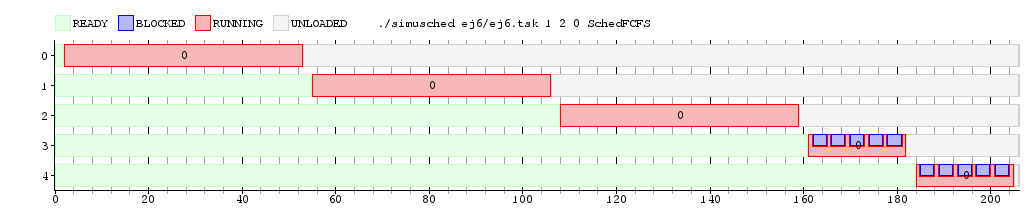
\includegraphics[width=\textwidth]{../ej6/ej6FCFS120.png}
  \caption{Tareas para Scheduler FCFS.}
  \label{fig:quant2}
\end{figure}

Analizando el gráfico y la salida análitica, llegamos a los siguientes valores:

\begin{table}[h!]
 	\begin{center}
 		\caption{Parámetros de calidad para el sceduler FCFS: SchedFCFS.}
 		\label{tab:table2}
 		\begin{tabular}{|l|c|c|c|c|c|}
 			\hline
 			& Tarea & Latencia & Waiting time & Total ejecución & Ratio (Espera/total) \\
 			\hline
 			\hline
 			\multirow{6}{*}{FCFS}
 			& 0 & 2 & 2 & 53 & 0.038 \\ \cline{2-6}
 			& 1 & 55 & 55 & 106 & 0.519 \\ \cline{2-6}
 			& 2 & 108 & 108 & 159 & 0.679 \\ \cline{2-6}
 			& 3 & 161 & 176 & 182 & 0.967 \\ \cline{2-6}
 			& 4 & 184 & 199 & 205 & 0.971 \\ \cline{2-6}
 			& Avg & 102 & 108 & 141 & 0.635 \\
 			\hline
 			
 		\end{tabular}
 	\end{center}
 \end{table}
 
Puede verse de estos valores que, por un lado, en los procesos que tienen sólo uso de CPU el ''waiting time'' es igual a la latencia, mientras que en aquellos que hacen utilización de recursos de entrada/salida el ''waiting time'' es igual a la latencia más el tiempo que la tarea permanece bloqueada.

Comparando las tablas \ref{tab:table1} y \ref{tab:table2} puede verse que en promedio la latencia empeora utilizando Scheduler FCFS en comparación con el Scheduler Round-Robin.

Respecto al ''waiting time'', el mismo mejora en promedio con respecto a todos los quanta probados con el Scheduler Round Robin, excepto para el caso de tareas con utilización de recursos de entrada/salida cuando el quantum es igual a 2.

La diferencia entre un Scheduler Round Robin y un Scheduler FCFS es más notoria respecto a las tareas con utilización de recursos de entrada/salida, dado que cuando no se realizan llamadas bloqueantes un Scheduler FCFS es un Scheduler Round Robin llevado al extremo, esto es, con un quantum lo suficientemente grande para que se pueda ejecutar cada tarea dentro del quantum asignado. Cuando se tienen en cuenta las tareas que hacen entrada/salida, puede verse que en realidad FCFS desfavorece dichos procesos pues desperdicia ciclos de CPU esperando el desbloqueo, mientras que un Scheduler Round Robin, aprovecha para cambiar el contexto y otorgar CPU a otra tarea. Pensando en un extremo en el que la entrada/salida bloquea al CPU durante muchos ciclos, puede concluirse que el Scheduler que más favorece este tipo de tareas es el Scheduler Round Robin con quantum pequeño.